\section{2019-10-30}
Recall the notions: hyperplane, half-space, polyhedron,
feasible regions of LPs, convex sets, extreme points
of convex sets.

\begin{thmbox}
    \subsection{Proposition}
    Let $ S\subseteq \mathbb{R}^n $ be a convex set and $ \bar{x}\in S $. 
    $ \bar{x} $ is an extreme point of $ S $ if and only if
    $ S\setminus \{\bar{x}\} $ is convex.
\end{thmbox}
\begin{proof}
    Assume $ S\subseteq\mathbb{R}^n $ is convex and $ \bar{x}\in S $.

    $\Rightarrow$
    Suppose $ \bar{x} $ is an extreme point of $ S $. Pick two points
    $ x^{(1)},x^{(2)}\in S\setminus\{\bar{x}\} $ and $ \lambda\in[0,1] $
    and set $\bar{x}=\lambda x^{(1)} + (1-\lambda)x^{(2)}$. To show
    that $ S\setminus\{\bar{x}\} $ is convex, we have to verify that $ x\in S\setminus\{\bar{x}\} $.
    Now the set $ S $ is convex, so $ x\in S $. It remains to show that
    $ x\neq \bar{x} $.

    Case 1: $ \lambda =0 $. Then $ x=x^{(1)}\neq \bar{x} $.

    Case 2: $ \lambda =1 $. Then $ x=x^{(2)}\neq \bar{x} $.

    Case 3: $ \lambda\in(0,1) $. We know $ x $ must be different from
    $ \bar{x} $, otherwise we would contradict the fact that $ \bar{x} $ is
    an extreme point of $ S $.

    $ \Leftarrow $ We prove the contrapositive. Assume that $ \bar{x} $
    is not an extreme point of $ S $. Then there exists two points
    $ x^{(1)},x^{(2)}\in S $ with $ x^{(1)}\neq x^{(2)} $ and some
    $ \lambda\in(0,1) $ such that $\bar{x}=\lambda x^{(1)} + (1-\lambda)x^{(2)}$.
    Note that $ x^{(1)},x^{(2)}\in S\setminus\{\bar{x}\}$ since
    $ x^{(1)}\neq x^{(2)} $. Thus $ S\setminus\{\bar{x}\} $ is not convex.
\end{proof}

\begin{defbox}
    \subsection{Definition (Tight Constraints)}
    Let $ A\in \mathbb{R}^{m \times n} $, $ \bm{b}\in \mathbb{R}^m $. Consider
    the polyhedron $ P\subseteq \mathbb{R}^n $
    $ P:=\{\bm{x}\in\mathbb{R}^n:A\bm{x}\le \bm{b}\} $. We say
    that a constraint $ \bm{\alpha ^\top} \bm{x}\le \beta $ of
    $ A \bm{x}\le \bm{b} $ is \emph{tight} for $ \bm{\bar{x}} $ if
    $ \bm{\alpha}^\top \bm{\bar{x}}=\beta $. We denote the set of all
    inequalities of $ A \bm{x}\le \bm{b} $ that
    are tight at $ \bm{\bar{x}} $ by $ A^=\bm{\bar{x}}=b^= $.
\end{defbox}


\begin{thmbox}
    \subsection{Theorem}
    Let $ P=\{\bm{x}\in\mathbb{R}^n:A \bm{x}\le \bm{b}\} $ be 
    a polyhedron and let $ \bm{\bar{x}}\in P $. 
    Let $ A^=\bm{x} = \bm{b}^= $ be the set of tight constraints
    for $ \bm{\bar{x}} $. 
    Then $ \rank(A^=)=n $ if and only if
    $\bm{\bar{x}}$ is an extreme point of $ P $.
\end{thmbox}

\begin{proof}
    $ \implies $ [$\rank(A^=)=n$ $ \implies $ $\bm{\bar{x}}$ is an extreme point of $ P $]
    
    Suppose $ \rank(A^=)=n $. Suppose for a contradiction that
    $\bm{\bar{x}}$ is not an extreme point. Then there exists
    $ \bm{x^{(1)}}, \bm{x^{(2)}}\in P$, where
    $ \bm{x^{(1)}} \neq \bm{x^{(2)}} $ and $ \lambda\in(0,1) $
    such that
    \[ \bm{\bar{x}}=\lambda \bm{x^{(1)}}+(1-\lambda)\bm{x^{(2)}}\]
    Thus,
    \begin{align*}
        \bm{b^=}&=A^=\bm{\bar{x}}\\
        &=A^=[\lambda \bm{x^{(1)}}+(1-\lambda)\bm{x^{(2)}}]\\
        &=\underbrace{\lambda}_{>0}
        \underbrace{A^=\bm{x^{(1)}}}_{\le \bm{b^=}}
        +\underbrace{(1-\lambda)}_{>0} 
        \underbrace{A^=\bm{x^{(2)}}}_{\le \bm{b^=}}\\
        &\le\lambda\bm{b^=}+(1-\lambda)\bm{b^=}\\
        &=\bm{b^=}
    \end{align*}
    Thus, we must have that everything in the inequality chain
    starting and ending with $ \bm{b^=} $ is equal. Thus,
    $ A^=\bm{x^{(1)}}=A^=\bm{x^{(2)}}=\bm{b^=}$.
    $ \rank(A^=)=n $ implies there is a unique solution
    to $ A^=\bm{\bar{x}}=\bm{b^=}$, so we have 
    $ \bm{\bar{x}}=\bm{x^{(1)}}=\bm{x^{(2)}} $, a contradiction that
    $ \bm{\bar{x}} $ is an extreme point.

    $ \impliedby $ [$\rank(A^=)=n$ $ \impliedby $ $\bm{\bar{x}}$ is an extreme point of $ P $]

    We will prove the contrapositive of this. That is, we will be prove
    $ \rank(A^=)\neq n $ $\implies$ $\bm{\bar{x}}$ is not 
    an extreme point of $ P $.

    Suppose that $ \rank(A^=)\neq n $, that is $ \rank(A^=)<n $, which
    means that the columns of $ A^= $ are linearly dependent. Thus,
    $ \exists \bm{d} $ such that $ A^=\bm{d}=\bm{0} $. Let
    $ \varepsilon > 0 $ be arbitrarily small and define
    \[ \bm{x^{(1)}} := \bm{\bar{x}} + \varepsilon \bm{d} \]
    \[ \bm{x^{(2)}} := \bm{\bar{x}} - \varepsilon \bm{d} \]
Hence, $ \bm{\bar{x}}=\frac{1}{2}\bm{x^{(1)}}+\frac{1}{2} \bm{x^{(2)}} $, where
$ \bm{x^{(1)}} $ and $ \bm{x^{(2)}} $ are distinct. Thus,
$ \bm{\bar{x}} $ is in the line segment between $ \bm{x^{(1)}} $ and
$ \bm{x^{(2)}} $. 

We need to show that $ \bm{x^{(1)}},\bm{x^{(2)}}\in P $
for  $ \varepsilon > 0 $ arbitrarily small. We have
\begin{align*}
    A^= \bm{x^{(1)}}&=A^=(\bm{\bar{x}} + \varepsilon \bm{d})\\
    &=A^= \underbrace{\bm{\bar{x}}}_{=\bm{b^=}}
    +\varepsilon\underbrace{A^= \bm{d}}_{=\bm{0}}\\
    &=\bm{b^=}
\end{align*}
Similarly, $ A^= \bm{x^{(2)}}= \bm{b^=}$. Let $ \bm{a}^\top \bm{x}\le \beta $
be any of the inequalities of $ A \bm{x}\le \bm{b} $ that is not in
$ A^= \bm{x}\le \bm{b}^= $. 
It follows for $ \varepsilon >0 $ arbitrarily small that:
\begin{align*}
    \bm{a}^\top \bm{x^{(1)}}&= \bm{a}^\top(\bm{\bar{x}} + \varepsilon \bm{d})\\
    &=\underbrace{\bm{a}^\top \bm{\bar{x}}}_{\le \beta}+
    \varepsilon \bm{a}^\top \bm{d}\\
    &\le \beta
\end{align*}
hence $ \bm{x^{(1)}}\in P $. Similarly, $ \bm{x^{(2)}}\in P $. Thus, 
$ \bm{\bar{x}} $ is properly contained in $ P $ and hence is not
an extreme point.
\end{proof}

\subsection{Example}
\[ F:=\left\{ \bm{x}\in\mathbb{R}^2: \begin{bmatrix}
    1 & 1\\
    1 & 0\\
    -1 & 0\\
    0 & -1
\end{bmatrix}\bm{x}\le
\begin{bmatrix}
    4\\
    2\\
    0\\
    0\\
\end{bmatrix}, \bm{x}\ge \bm{0} \right\} \]
(i) 
$\bm{x}^{(1)}:=\begin{bmatrix}2\\0\end{bmatrix}$,
$ A^= =
\begin{bmatrix}
    1 & 0\\
    0 & -1
\end{bmatrix} $

$ \rank(A^=)=2=n $, therefore $\bm{x}^{(1)}$ is an extreme
point of $ F $.

(ii)
$\bm{x}^{(2)}:=\begin{bmatrix}2\\2\end{bmatrix}$,
$ A^= =
\begin{bmatrix}
    1 & 1\\
    1 & 0
\end{bmatrix} $

$ \rank(A^=)=2=n $, therefore $\bm{x}^{(2)}$ is an extreme
point of $ F $.

(iii)
$\bm{x}^{(3)}:=\begin{bmatrix}2\\1\end{bmatrix}$,
$ A^= =
\begin{bmatrix}
    1 & 0
\end{bmatrix} $

$ \rank(A^=)=1<2=n $, therefore $\bm{x}^{(3)}$ is not an extreme
point of $ F $.

\begin{center}
    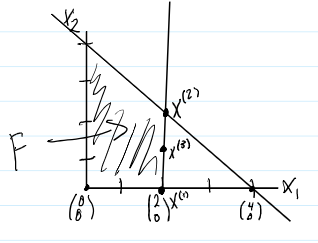
\includegraphics{tightsolns}
\end{center}

\begin{thmbox}
    \subsection{Theorem}
    Let $ A\in\mathbb{R}^{m\times n} $ with $ \rank(A)=m $. 
    Let $ P=\{\bm{x}\in\mathbb{R}^n: A \bm{x}=\bm{b},
    \bm{x}\ge \bm{0}\} $, and let $ \bm{\bar{x}}\in P $.
    $ \bm{\bar{x}} $ is an extreme point of $ P $ if and only if $ \bm{\bar{x}} $ is a basic feasible solution of $  A \bm{x}=\bm{b} $.
\end{thmbox}

\[ F:=\left\{ \bm{x}\in\mathbb{R}^2: \begin{bmatrix}
    1 & 1\\
    1 & 0\\
    -1 & 0\\
    0 & -1
\end{bmatrix}\bm{x}\le
\begin{bmatrix}
    4\\
    2\\
    0\\
    0\\
\end{bmatrix}, \bm{x}\ge \bm{0} \right\} \]

\[ P:=\left\{\bm{x}\in\mathbb{R}^4:
\begin{bmatrix}
    1&1&-1&0\\
    1&0&0&-1
\end{bmatrix}\bm{x}=
\begin{bmatrix}
    4\\
    2
\end{bmatrix}, \bm{x}\ge \bm{0}\right\} \]
Note that for every feasible solution
$ \begin{bmatrix}
    \bar{x_1}\\
    \bar{x_2}
\end{bmatrix}\in F $,
$ \begin{bmatrix}
    \bar{x_1}\\
    \bar{x_2}\\
    4-\bar{x_1}-\bar{x_2}\\
    2-\bar{x_1}
\end{bmatrix}\in P $.

Conversely, for every 
$ \begin{bmatrix}
    \hat{x_1}\\
    \hat{x_2}\\
    \hat{x_3}\\
    \hat{x_4}
\end{bmatrix}\in P $,
$ \begin{bmatrix}
    \hat{x_1}\\
    \hat{x_2}
\end{bmatrix}\in F $

Consider the basis $ B:=\{3,4\} $ of $ A $. The corresponding basic feasible
solution is $ \bm{\bar{x}}=(0,0,4,2)^\top $. Thus, $ \bm{\bar{x}} $ is
an extreme point of $ P $.

\subsection{Geometric Interpretation of Simplex Method}
(P)
\[ \max z:=\bm{c}^\top x \]
subject to
\[ A \bm{x}\le \bm{b} \]
\[ \bm{x}\ge \bm{0} \]
Suppose $ n=1 $ and $ m=6 $ with $ \bm{b}\ge \bm{0} $.

\begin{center}
    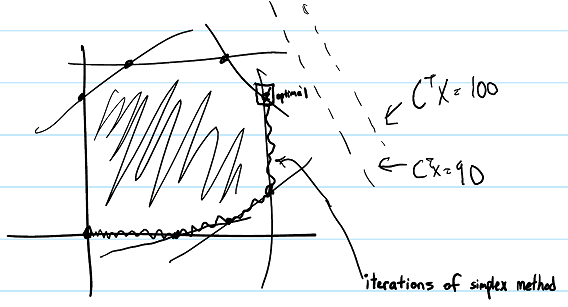
\includegraphics{geosimplex}
\end{center}

\subsection{Duality Theory}
(P)
\[ \max \{\bm{c}^{\top} \bm{x}: A \bm{x}=\bm{b},\, \bm{x} \geq \bm{0}\} \]
Recall the notation of optimality certificate $ \bm{\bar{y}}\in\mathbb{R}^m $ such that $ A ^\top \bm{\bar{y}}\ge \bm{c} $. We noted that for
every feasible $ \bm{x} $ in (P), $ A \bm{x}= \bm{b}\implies
\bm{\bar{y}}^\top A \bm{x}=\bm{\bar{y}}^\top \bm{b} $

Since $ A ^\top \bm{\bar{y}}\ge \bm{c} $ and $ \bm{x}\ge \bm{0} $,
we have $ \bm{c}^\top \bm{x}\le \bm{\bar{y}}^\top A \bm{x} =
\bm{\bar{y}}^\top \bm{b} $. So as long as $ \bm{y}\in\mathbb{R}^m $
with $ A ^\top \bm{y}\ge \bm{c} $, we can get an upper bound
of $ \bm{b} ^\top\bm{y} $ on the optimal objective value of (P).

We want to minimize $ \bm{b}^\top\bm{y} $ subject to $ A ^\top \bm{y}\ge \bm{c} $

\begin{defbox}
    \subsection{Definition (Dual)}
    Given (P)
    \[ \max \{\bm{c}^{\top} \bm{x}: A \bm{x}=\bm{b},\, \bm{x} \geq \bm{0}\} \]
    we define (D)
    \[ \min \{\bm{b}^{\top} \bm{y}: A^{\top} \bm{y} \geq \bm{c},\, \bm{y} \geq \bm{0}\}\]
    to be the \emph{dual} of (P).
\end{defbox}

\subsection{Example (Dual)}
Find the dual of
$ (P_1)$: $\max \{\bm{c}^\top \bm{x}: A \bm{x}\le \bm{b},\,\bm{x}\ge \bm{0}\}$.

\emph{Solution.}

Convert to SEF by introducing slack variables: $ \bm{s}=(s_1,\ldots,s_n)^\top $.

$ (P_2) $
\[ \max \bm{c}^\top
\begin{bmatrix}
    \bm{x}\\
    \bm{s}
\end{bmatrix} \]
subject to
\[ \left[ \begin{array}{c|c}
    A & I
\end{array} \right]
\begin{bmatrix}
    \bm{x}\\
    \bm{s}
\end{bmatrix} = \bm{b} \]
\[ (\bm{x},\bm{s})^\top\ge \bm{0} \]

$ (D_2) $
\[ \min \bm{b}^\top \bm{y} \]
\[ \begin{bmatrix}
    A^T\\
    I
\end{bmatrix} \ge
\begin{bmatrix}
    \bm{c}\\
    \bm{0}
\end{bmatrix}\]
\[ \bm{y}\ge \bm{0} \]

Thus, the dual of $ (P_1) $ is $ (D_2) $: 
$\min\{\bm{b}^\top \bm{y}: A ^\top \bm{y}\ge \bm{c},\,\bm{y}\ge \bm{0}\}$.